\documentclass[a4paper,12pt]{article}
\usepackage[left=2.5cm,right=2.5cm,top=2.5cm,bottom=2.5cm]{geometry} % Adjust page margins
\usepackage{xcolor,graphicx,framed}
\usepackage[normalem]{ulem}
\usepackage{amsmath}
\usepackage{cases}
\usepackage{gensymb}
\usepackage{chemmacros}
\setlength{\extrarowheight}{0.4cm}

\begin{document}

\newcommand{\HRule}{\rule{\linewidth}{0.4mm}} % Defines a new command for the horizontal lines, change thickness here

%----------------------------------------------------------------------------------------
%	HEADING SECTIONS
%----------------------------------------------------------------------------------------

\begin{minipage}{0.7\textwidth}
\begin{flushleft} 
\textsc{Universidad del Valle de Guatemala \\
Campus Central \\
Facultad de Ciencias y Humanidades \\
Departamento de Qu\'imica \\
Segundo ciclo, 2014 \\
Fisicoqu\'imica 1 \\
}
\end{flushleft}
\end{minipage}
~
\begin{minipage}{0.2\textwidth}
\begin{flushright}

\includegraphics[scale=0.3]{Logo_UVG} % Include a department/university logo
\end{flushright}
\end{minipage}\\

%----------------------------------------------------------------------------------------
%	TITLE SECTION
%----------------------------------------------------------------------------------------

\begin{center}
\HRule \\[0.4cm]
{ \bfseries Soluciones propuestas a los ejercicios en clase, 12}\\ % Title of your document
\HRule \\[0.4cm]
\end{center}

%----------------------------------------------------------------------------------------

\begin{enumerate}

 \item \textbf{\textit{(Chang 7.55)} Los vol\'umenes molares parciales de una soluci\'on benceno-tetracloruro de carbono a $25\celsius$ a una fracci\'on molar de 0.5 son: $V_b=0.106\;\mbox{L}\cdot\mbox{mol}^{-1}$ y $V_c=0.100\;\mbox{L}\cdot\mbox{mol}^{-1}$, respectivamente, donde los sub\'indice b y c denotan $\mbox{C}_6\mbox{H}_6$ y $\mbox{CCl}_4$}.
 \begin{enumerate}
  \item \textbf{?`Cu\'al es el volumen de la soluci\'on formada por un mol de cada uno de ellos?}

Usando los vol\'umenes parciales molares de los componentes, el volumen viene dado por:
$$V=n_bV_b+n_cV_c=(1\;\mbox{mol})(0.106\;\mbox{L}\cdot\mbox{mol}^{-1})+(1\;\mbox{mol})(0.100\;\mbox{L}\cdot\mbox{mol}^{-1})=0.206\;\mbox{L}$$

  \item \textbf{Dado que los vol\'umenes molares son $\mbox{C}_6\mbox{H}_6=0.089\;\mbox{L}\cdot\mbox{mol}^{-1}$ y $\mbox{CCl}_4=0.097\;\mbox{L}\cdot\mbox{mol}^{-1}$, ?`cu\'al es el cambio de volumen al mezclar $1\;\mbox{mol}$ de cada uno de ellos ($\mbox{C}_6\mbox{H}_6$ y $\mbox{CCl}_4$)?}

El volumen antes de mezclar que ten\'ia el benceno es: 
$$V_b=\bar{V}_b\cdot n_b=(0.089\;\mbox{L}\cdot\mbox{mol}^{-1})(1\;\mbox{mol})=0.089\;\mbox{L}$$ 
Y el que ten\'ia el tetracloruro es: 
$$V_c=\bar{V}_c\cdot n_c=(0.097\;\mbox{L}\cdot\mbox{mol}^{-1})(1\;\mbox{mol})=0.097\;\mbox{L}$$
As\'i que el volumen total antes de mezclarlos era:
$$V_{antes}=V_b+V_c=0.089\;\mbox{L}+0.097\;\mbox{L}=0.186\;\mbox{L}$$
Por lo que el cambio de volumen al mezclarlos es:
$$\Delta V=V-V_{antes}=0.206\;\mbox{L}-0.186\;\mbox{L}=0.020\;\mbox{L}$$

  \item \textbf{?`Qu\'e puede deducir acerca de la naturaleza de las fuerzas intermoleculares entre el $\mbox{C}_6\mbox{H}_6$ y el $\mbox{CCl}_4$?}

Como se tiene m\'as volumen al mezclarlos que antes, las fuerzas intermoleculares entre el benceno y el tetracloruro de carbono son de repulsi\'on, es decir, necesitan m\'as volumen al mezclarlos porque se repelen (comparado con las fuerzas intermoleculares en las soluciones puras).

 \end{enumerate} % Problema 7.55 de Chang

 \item \textbf{\textit{(Chang 7.58)} Suponga que se mezclan $2.6\;\mbox{moles}$ de $\mbox{He}$ a $0.80\;\mbox{atm}$ y $25\celsius$ con $4.1\;\mbox{moles}$ de $\mbox{Ne}$ a $2.7\;\mbox{atm}$ y $25\celsius$. Calcule el cambio de la energ\'ia de Gibbs del proceso. Suponga un comportamiento ideal.} % Problema 7.58 de Chang

N\'otese que los gasese no est\'an a la misma presi\'on, por lo que al mezclarlos hay dos contribuciones, una por la mezcla y otra por los cambios de presi\'on. Ambas las podemos calcular con la ecuaci\'on:
$$\Delta_{mix}G=n_{He}RT\times\ln\frac{P_{He,mezcla}}{P_{He,antes}}+n_{Ne}RT\times\ln\frac{P_{Ne,mezcla}}{P_{Ne,antes}}$$
Para determinar la presi\'on parcial de cada gas luego de mezclarlos, necesitamos la presi\'on total luego de mezclarlos. Asumiendo un comportamiento ideal, podemos determinarla a partir del volumen total y los moles totales luego de mezclar. 
El volumen del $\mbox{He}$ (a $T=25+273.15=298.15\;\mbox{K}$), antes de mezclarlo, es:
$$V_{He}=\frac{n_{He}RT}{P_{He,antes}}=\frac{(2.6\;\mbox{moles})(0.0821\;\mbox{L}\cdot\mbox{atm}\cdot\mbox{K}^{-1}\cdot\mbox{mol}^{-1})(298.15\;\mbox{K})}{0.80\;\mbox{atm}}=79.6\;\mbox{L}$$
Mientras que el de $\mbox{Ne}$ es:
$$V_{Ne}=\frac{n_{Ne}RT}{P_{Ne,antes}}=\frac{(4.1\;\mbox{moles})(0.0821\;\mbox{L}\cdot\mbox{atm}\cdot\mbox{K}^{-1}\cdot\mbox{mol}^{-1})(298.15\;\mbox{K})}{2.7\;\mbox{atm}}=37.2\;\mbox{L}$$
Entonces el volumen total al mezclarlos es:
$$V_{total}=V_{He}+V_{Ne}=79.6\;\mbox{L}+37.2\;\mbox{L}=116.7\;\mbox{L}$$
Adem\'as, como tenemos que $n_{total}=n_{He}+n_{Ne}=2.6\;\mbox{moles}+4.1\;\mbox{moles}=6.7\;\mbox{moles}$, entonces:
$$P_{total}=\frac{n_{total}RT}{V_{total}}=\frac{(6.7\;\mbox{moles})(0.0821\;\mbox{L}\cdot\mbox{atm}\cdot\mbox{K}^{-1}\cdot\mbox{mol}^{-1})(298.15\;\mbox{K})}{116.7\;\mbox{L}}=1.41\;\mbox{atm}$$
Las presiones parciales luego de mezclarlos las podemos determinar por medio de las fracciones molares que son:
$$x_{He}=\frac{n_{He}}{n_{total}}=\frac{2.6\;\mbox{moles}}{6.7\;\mbox{moles}}=0.39$$
Y:
$$x_{Ne}=\frac{n_{Ne}}{n_{total}}=\frac{4.1\;\mbox{moles}}{6.7\;\mbox{moles}}=0.61$$
As\'i que:
$$P_{He,mezcla}=x_{He}\cdot P_{total}=(0.39)(1.41\;\mbox{atm})=0.55\;\mbox{atm}$$
Y:
$$P_{Ne,mezcla}=x_{Ne}\cdot P_{total}=(0.61)(1.41\;\mbox{atm})=0.86\;\mbox{atm}$$
Entonces el cambio de la energ\'ia de Gibbs para la mezcla es:

\begin{tabular}{r c l}
$\Delta_{mix}G$ & $=$ & $RT(n_{He}\times\ln\frac{P_{He,mezcla}}{P_{He,antes}}+n_{Ne}\times\ln\frac{P_{Ne,mezcla}}{P_{Ne,antes}})$ \\
& $=$ & $(8.314\;\mbox{K}\cdot\mbox{K}^{-1}\cdot\mbox{mol}^{-1})(298.15\;\mbox{K})\left((2.6\;\mbox{moles})\ln\frac{0.55\;\mbox{atm}}{0.80\;\mbox{atm}}\right.$ \\
& & $\;\;+\left.(4.1\;\mbox{moles})\ln\frac{0.86\;\mbox{atm}}{2.7\;\mbox{atm}}\right)$ \\
& $=$ & $-14.1\;\mbox{kJ}$
\end{tabular}

 \item \textbf{\textit{(Chang 7.11)} A $25\celsius$ y $1\;\mbox{atm}$ de presi\'on, las entrop\'ias absolutas de la tercera ley para el metano y el etano son $186.19\;\mbox{J}\cdot\mbox{K}^{-1}\cdot\mbox{mol}^{-1}$ y $229.49\;\mbox{J}\cdot\mbox{K}^{-1}\cdot\mbox{mol}^{-1}$, respectivamente, en la fase gaseosa. Calcule la entrop\'ia absoluta de tercera ley para una soluci\'on que contiene $1\;\mbox{mol}$ de cada gas. Suponga un comportamiento ideal.} % Problema 7.11 de Chang

La entrop\'ia absoluta de tercera ley para la soluci\'on ser\'ia la entrop\'ia antes de mezclarlos m\'as el cambio de entrop\'ia de la mezcla. \'Esta \'ultima se puede determinar a partir de:
$$\Delta_{mix}S=-nR(x_1\ln x_1+x_2\ln x_2)$$
En este caso, como son $1\;\mbox{mol}$ de cada gas, entonces $n=2\;\mbox{mol}$ y $x_{metano}=x_{etano}=n_i/n=(1\;\mbox{mol})/(2\;\mbox{mol}=0.5$, entonces:
$$\Delta_{mix}S=-(2\;\mbox{mol})(8.314\;\mbox{J}\cdot\mbox{K}^{-1}\cdot\mbox{mol}^{-1})((0.5)\ln 0.5+(0.5)\ln 0.5)=11.53\;\mbox{J}\cdot\mbox{K}^{-1}$$
As\'i que la entrop\'ia absoluta de la tercera ley es:

\begin{tabular}{r c l}
$S$ & $=$ & $S_{metano}+S_{etano}+\Delta_{mix}S$ \\
& $=$ & $(1\;\mbox{mol})(186.19\;\mbox{J}\cdot\mbox{K}^{-1}\cdot\mbox{mol}^{-1})+(1\;\mbox{mol})(229.49\;\mbox{J}\cdot\mbox{K}^{-1}\cdot\mbox{mol}^{-1})$ \\
& & $\;\;+11.53\;\mbox{J}\cdot\mbox{K}^{-1}$ \\
& $=$ & $427.21\;\mbox{J}\cdot\mbox{K}^{-1}$
\end{tabular}

 \item \textbf{\textit{(Chang 7.14)} La constante de la ley de Henry para ox\'igeno en el agua a $25\celsius$ es de $773\;\mbox{atm}\cdot\mbox{mol}^{-1}\cdot\mbox{kg}$ de agua. Calcule la molalidad del ox\'igeno en el agua a una presi\'on parcial de $0.20\;\mbox{atm}$. Suponiendo que la solubilidad del ox\'igeno en la sangre a $37\celsius$ es aproximadamente la misma que en agua a $25\celsius$, comente sobre la esperanza de sobrevivencia humana sin mol\'eculas de hemoglobina. (El volumen total de sangre en el cuerpo humano es aproximadamente de $5\;\mbox{L}$.)} % Problema 7.13 de Chang

Por la ley de Henry, tenemos que:
$$P_{O_2}=K_{O_2}'m$$
Entonces, la molalidad del ox\'igeno en el agua a $25\celsius$ es:
$$m=\frac{P_{O_2}}{K_{O_2}'}=\frac{0.20\;\mbox{atm}}{773\;\mbox{atm}\cdot\mbox{mol}^{-1}\cdot\mbox{kg}}=2.6\times 10^{-4}\;\mbox{mol}\cdot\mbox{kg}^{-1}$$

%Aunque tengamos $5\;\mbox{L}$ de sangre, la concentraci\'on del ox\'igeno es muy baja como para que simplemente por solubilidad en la sangre, podamos proveer de la cantidad de ox\'igeno necesario para la sobrevivencia humana. (Se recomienda buscar valores de concentraciones de ox\'igeno necesarias en el cuerpo humano.)

 \item \textbf{\textit{(McQuarrie 24-19)} El tetraclorometano y el tricloroetileno forman una solución esencialmente ideal a $40\celsius$ para cualquier concentración. Las presiones de vapor a $40\celsius$ son $214\;\mbox{torr}$ y $138\;\mbox{torr}$, respectivamente. La presi\'on total en t\'erminos de $x_2$ viene dada por:
$$P=x_1P_1^\star+x_2P_2^\star=(1-x_2)P_1^\star+x_2P_2^\star=P_1^\star+x_2(P_2^\star-P_1^\star)$$
Determinar $y_2$ en funci\'on de $x_2$ (incluyendo las constantes $P_1^\star$ y $P_2^\star$). Despejar $x_2$ y sustituirlo en la ecuaci\'on anterior. Usar este resultado para construir el diagrama de presi\'on-composici\'on de esta soluci\'on.} % Problema 10-19

La fracci\'on molar del tricloroetileno en la fase de vapor, $y_2$, puede ser determinada por medio de la ley de Dalton de presiones parciales, con la que se tiene que:
$$y_2=\frac{P_2}{P}=\frac{x_2P_2^\star}{P_1^\star+x_2(P_2^\star-P_1^\star)}$$
Despejando $x_2$:
$$y_2(P_1^\star+x_2(P_2^\star-P_1^\star))=x_2P_2^\star\;\Rightarrow\;y_2P_1^\star+y_2x_2(P_2^\star-P_1^\star)=x_2P_2^\star$$
$$\Rightarrow\;y_2P_1^\star=x_2P_2^\star-y_2x_2(P_2^\star-P_1^\star)\;\Rightarrow\;y_2P_1^\star=x_2(P_2^\star-y_2(P_2^\star-P_1^\star))$$
$$\Rightarrow\;x_2=\frac{y_2P_1^\star}{P_2^\star-y_2(P_2^\star-P_1^\star)}$$
Sustituyendo en $x_2$ en la ecuaci\'on de la presi\'on de vapor total:
$$P=P_1^\star+\left(\frac{y_2P_1^\star}{P_2^\star-y_2(P_2^\star-P_1^\star)}\right)(P_2^\star-P_1^\star)=\frac{P_1^\star P_2^\star}{P_2^\star+y_2(P_1^\star-P_2^\star)}$$

Entonces, el diagrama de presi\'on-composici\'on de la soluci\'on a $40\celsius$ es:

\begin{center}
 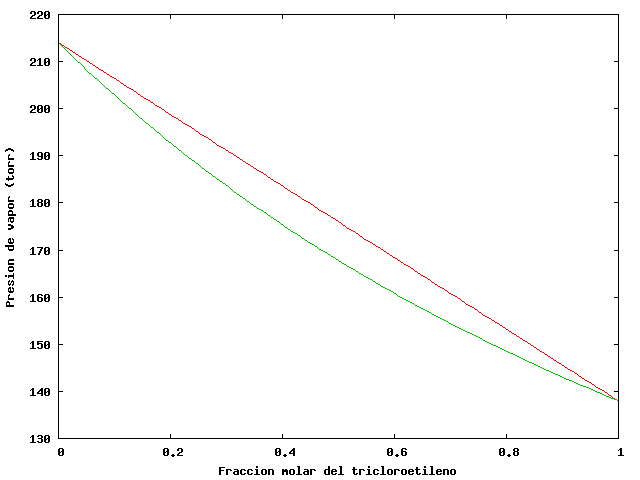
\includegraphics[scale=0.8]{figure10.png}
\end{center}

\end{enumerate}

\end{document}
